
\chapter{The Serre Equations}
\label{chp:Serreeqns}

%The Serre equations are partial differential equations that describe the behaviour of waves of free surface flows of fluids for a wide array of wave properties. 

%spectrum of wave models%



%In fact they are considered to be one of the best models for free surface flows up to wave breaking []. For  this reason we are interested in using the Serre equations to model wave hazards such as tsunamis and storm surges. 

%The Serre equations can be derived asymptotically [] or via depth integration [] of the full Navier-Stokes equations. They are evolution type equations, however they are not strictly parabolic or hyperbolic and naively are not in conservation law form.  


% Introduce Serre Equations/ Conservative/ Non-conservative, Non-dimensionalised
% Properties : Conservation of Mass, Energy and Momentum, Dispersion relation, wave speed bounds, Analytic solutions

%Use properties to asess numerical methods

\section{The Equations}
%[!]-----[!] DISPERSION!!!!!
%full nonlineariy, good approximation to Euler equations up to wave breaking
There are three primary ways in which the Serre equations have been derived from the Euler equations in the literature; by asymptotic expansion \cite{Serre-F-1953-857,Bonneton-Lannes-2009-16601}, directed fluid sheets \cite{Green-Naghdi-1976-237} and depth integration \cite{Su-Gardener-1969-536,Zoppou-2014}. In this thesis the depth integration view of the equations is taken, although the derivation is omitted given the extent of literature already available. 

From the depth-integration approach the Serre equations describe a free surface fluid defined by its height $h(x,t)$ above a stationary bed profile $b(x)$ with depth average of its horizontal velocity $u(x,t)$ as in Figure \ref{fig:WaterModel}. The derivation is similar to that of the Shallow Water Wave Equations (SWWE) [], except for the Serre equations the vertical velocity $v(x,z,t)$ varies linearly with depth and is given by []
\begin{equation}
v(x,z,t) = u \frac{\partial b}{\partial x} - (z - b) \frac{\partial u}{\partial x}.
\label{eqn:VertVelSerre}
\end{equation}
Because the vertical velocity of the Serre equations is not $0$ throughout the depth of water as in the SWWE, the Serre equations possess a non-hydrostatic pressure distribution.

\begin{figure}
	\centering
	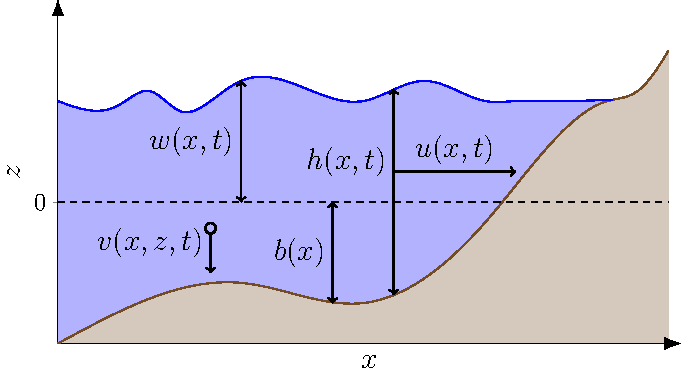
\includegraphics[width=\textwidth]{./chp2/figures/SerreModel.pdf}
	\caption{Diagram demonstrating the quantities used to describe the fluid (\squareF{blue}) and the bed (\squareF{brown!80!black}) for the Serre equations.}
	\label{fig:WaterModel}
\end{figure}

By depth integrating the Euler equations [] with a no-slip condition at the bed and a free surface condition at the free surface we obtain the depth integrated approximation of the conservation of mass and momentum equations
\begin{subequations}
	\begin{align}
	&\frac{\partial h}{\partial t} + \dfrac{\partial (uh)}{\partial x} = 0,  \label{eqn:FullSerreNonConMass} \\ \nonumber \\
	&\dfrac{\partial (uh)}{\partial t} + \dfrac{\partial}{\partial x} \left ( u^2h + \dfrac{gh^2}{2} + \dfrac{h^2}{2}{\Psi} + \dfrac{h^3}{3}{ \Phi }  \right )  +  \dfrac{\partial b}{\partial x} \left (gh +   h \Psi + \dfrac{h^2}{2}{ \Phi }  \right ) = 0	\label{eqn:FullSerreNonConMome}
	\end{align}
	\label{eqn:FullSerreNonCon}
\end{subequations}
where the $\Phi$ and $\Psi$ terms account for the non-hydrostatic part of the pressure and are
	\begin{subequations}
	\begin{align}
	{ \Psi }  &= \dfrac{\partial b}{\partial x}\left(\dfrac{\partial u}{\partial t} + u\dfrac{\partial u}{\partial x} \right)  + u^2\dfrac{\partial^2 b}{\partial x^2}, \label{eqn:SerreeqnPsi} \\ \nonumber \\
 { \Phi }  &= \dfrac{\partial u }{\partial x} \dfrac{\partial u}{\partial x} -u \dfrac{\partial^2 u}{\partial x^2}  - \dfrac{\partial^2 u}{\partial x \partial t} . \label{eqn:SerreeqnPhi} 
	\end{align}
	\label{eqn:FullSerreNonConVarDef}
	\end{subequations}
When $\Phi = \Psi = 0$ the Serre equations are equivalent to the SWWE where the vertical velocity is $0$, only the hydrostatic pressure is present and there is no dispersion. Due to the presence of the $\Phi$ and $\Psi$ terms the Serre equations are much more difficult to solve analytically and numerically than the SWWE. The primary reason for this is that whilst the SWWE are hyperbolic for finite water depth, the Serre equations are neither hyperbolic nor parabolic. Furthermore the Serre equations are not in conservation law form due to the presence of temporal derivatives in $\Phi$ and $\Psi$, although they are derived from conservation equations. 

For a horizontal bed $\partial b / \partial x = 0$, $\Psi = 0$ and so the Serre equations reduce to
\begin{subequations}
	\label{eqn:FullSerreNonConHorizbed}
	\begin{align}
	\label{eqn:FullSerreNonConMassHorizbed}
	&\frac{\partial h}{\partial t} + \dfrac{\partial (uh)}{\partial x} = 0, \\ \nonumber \\
	\label{eqn:FullSerreNonConMomeHorizbed}
	&\dfrac{\partial (uh)}{\partial t} + \dfrac{\partial}{\partial x} \left ( u^2h + \dfrac{gh^2}{2} + \dfrac{h^3}{3}{ \Phi }  \right ) = 0.
	\end{align}
\end{subequations}	
These equations are neither hyperbolic nor parabolic and are not in conservation law form as $\Phi$ contains a temporal derivative. As such even for horizontal beds the Serre equations are more challenging to solve analytically and numerically than the SWWE. 

\subsection{Alternative form of the Serre Equations}
A major hurdle for developing numerical methods for the Serre equations is the presence of the mixed temporal and spatial derivative in $\Phi$ and $\Psi$ \eqref{eqn:FullSerreNonConVarDef}. By rewriting the Serre  equations and introducing a new conserved quantity $G$ \cite{Hank-etal-2010-2034,Zoppou-2014,Li-2014-169}, the mixed temporal and spatial derivative can be removed and the Serre equations can be written in conservation law form.
\begin{defn}
	\label{defn:SerreEqnConservedQuantity1}
	The conserved quantity $G$ is
	\[ G =  h {u} \left(1 + \frac{\partial h}{\partial x}\frac{\partial b}{\partial x} + \frac{1}{2}h\frac{\partial^2 b}{\partial x^2} + \left[\frac{\partial b}{\partial x}\right]^2 \right) - \frac{\partial}{\partial x}\left(\frac{1}{3}h^3  \frac{\partial {u}}{\partial x}\right).\]
\end{defn}

The Serre equations \eqref{eqn:FullSerreNonCon} can then rewritten as conservation laws with a source term for the conserved variables $h$ and $G$
\begin{subequations}
	\label{eqn:FullSerreCon}
	\begin{align}
	& \frac{\partial h}{\partial t} + \dfrac{\partial (uh)}{\partial x} = 0 ,\label{eqn:FullSerreConMass}  \\ \nonumber \\
	\begin{split}
	\label{eqn:Serreconsconmom}
		\frac{\partial G}{\partial t}  + \frac{\partial}{\partial x} \left( {u} G + \frac{gh^2}{2} - \frac{2}{3}h^3 \left[\frac{\partial {u}}{\partial x}\right]^2 + h^2 {u}\frac{\partial {u}}{\partial x}\frac{\partial b}{\partial x} \right) \\ \\ + \frac{1}{2}h^2 {u} \frac{\partial {u}}{\partial x} \frac{\partial^2 b}{\partial x^2}  - h {u}^2\frac{\partial b}{\partial x}\frac{\partial^2 b}{\partial x^2} + gh\frac{\partial b}{\partial x} = 0.
	\end{split}
	\end{align}
\end{subequations}
The conserved quantity $G$ resembles $h$ multiplied by the irrotationality \cite{Choi-Camassa-1999-1,Carter-Cienfuegos-2011-259}.

This conservation law form makes the Serre equations well suited to be numerically solved using a finite volume method for the conservation of mass and $G$ equations, provided one can solve for $u$ given $h$ and $G$.

For a horizontal bed $\partial b / \partial x = 0$ the conservation law form of the Serre equations is
\begin{subequations}
	\label{eqn:FullSerreConHorizBed}
	\begin{align}
	&\frac{\partial h}{\partial t} + \dfrac{\partial (uh)}{\partial x} = 0, \label{eqn:FullSerreConMassHorizBed} \\  \nonumber \\
	&\frac{\partial G}{\partial t}   + \frac{\partial}{\partial x} \left( {u} G + \frac{gh^2}{2} - \frac{2}{3}h^3 \left[\frac{\partial {u}}{\partial x}\right]^2 \right) = 0 , \label{eqn:SerreconsconmomHorizBed}\\ \nonumber \\
	&G =  h {u}  - \frac{\partial}{\partial x}\left(\frac{1}{3}h^3  \frac{\partial {u}}{\partial x}\right). \label{defn:SerreEqnConservedQuantity1HorizBed}
	\end{align}
\end{subequations}


\section{Properties of the Serre Equations}
The Serre equations possess a number of properties that can be used to assess the veracity of numerical methods. Because if a numerical method approximates the Serre equations accurately then the properties of the numerical method should approximate the properties of the Serre equations. In this thesis the conservation properties, dispersion properties, analytic solutions of the Serre are employed and so are presented here. 

To complement the available analytic solutions, the Serre equations are modified to force certain analytic solutions using a source term, which are called forced solutions. These forced solutions will be used to assess the validity of the numerical methods for a wider array of flow scenarios then possible given the limited number of analytic solutions for the Serre equations.

Finally the results of \citet{Pitt-2017-1725} for the behaviour of the Serre equations in the presence of steep gradients are presented. These results satisfied one of the main objectives of the Thesis and contained behaviours that were not previously present in the literature. 

\subsection{Conservation Properties}
Conservation of a quantity means that in a closed system the total amount of a quantity $q$ remains constant in time.
\begin{defn}
	\label{defn:TotalAmmountab}
	The total amount of a quantity $q$ in a system occurring on the interval $[a,b]$ at time $t$ is
	\begin{equation*}
	\mathcal{C}_q(t) = \int_{a}^{b} q(x,t)\, dx.
	\end{equation*}
\end{defn}
Conservation of a quantity $q$ means that $\mathcal{C}_{q}(0) = \mathcal{C}_{q}(t)$ for all $t$. Given that the Serre equations \eqref{eqn:FullSerreNonCon} are conservation equations for mass and momentum and that the conservation of momentum equation can be rewritten as a conservation equation for $G$ \eqref{eqn:FullSerreCon}, the Serre equations conserve all these quantities. Additionally the Serre equations were derived by \citet{Green-Naghdi-1976-237} by conserving the energy $\mathcal{H}$
\begin{equation}
	\mathcal{H}(x,t) = \frac{1}{2} \left( g\left(h^2 + 2hb\right) + hu^2  + \frac{h^3}{3} \left(\frac{\partial u}{\partial x}\right)^2 + u^2h\left[\frac{\partial b}{\partial x}\right]^2 - uh^2 \frac{\partial u}{\partial x} \frac{\partial b}{\partial x}  \right).
	\label{eqn:Hamildef}
\end{equation}
The energy $\mathcal{H}$ is the sum of the gravitational potential energy, the horizontal kinetic energy and the vertical kinetic energy which over the depth of water are
\begin{align}
& \int_{b}^{h +b} gz \; dx = g\left(h^2 + 2hb\right), \\
& \int_{b}^{h +b} u^2 \; dx = hu^2, \\
& \int_{b}^{h +b} v^2 \; dx = \frac{h^3}{3} \left(\frac{\partial u}{\partial x}\right)^2 + u^2h\left[\frac{\partial b}{\partial x}\right]^2 - uh^2 \frac{\partial u}{\partial x} \frac{\partial b}{\partial x},
\end{align}
respectively. For horizontal beds $\mathcal{H}$ is also the Hamiltonian of the Serre equations \cite{Li-Y-2002}. 
 
For the system to be closed the flux terms of the conservation of mass and momentum equations at the boundaries must cancel and the integral of the source term over the domain must be zero.

\subsection{Dispersion Properties}
The dispersion properties of wave equations are primarily studied through linearising the equations, assuming periodic wave solutions and then deriving a relationship between the frequency $\omega$ and wave number $k$ of these solutions. For the Serre equations the dispersion relation [] is
\begin{equation}
\label{eqn:DispersionRelation}
\omega = Uk \pm k \sqrt{gH} \sqrt{\frac{3}{\left(kH\right)^2 + 3}}.
\end{equation}
\citet{Barthelemy-2004-315} compared this dispersion relation to that of the linear theory of water waves and demonstrated its utility when $k$ is small. However when $k$ is large the difference between the dispersion relation of the Serre equations and that of water wave theory increases. The dispersion relation of the Serre equations can be modified by introducing terms to reduce this difference \cite{Barthelemy-2004-315}, but such modifications are beyond the scope of this thesis.


From the dispersion relation \eqref{eqn:DispersionRelation} the phase velocity $v_p = \omega / k$  and the group velocity $v_g = \partial \omega / \partial  k$ can be written in terms of wave number as
\begin{subequations}
	\label{eqn:WaveVelocities}
	\begin{equation}
	\label{eqn:WaveVelocitiesPhase}
	v_p = U \pm \sqrt{gH}\sqrt{\frac{3}{\left(kH\right)^2 + 3}},
	\end{equation}
	\begin{equation}
	\label{eqn:WaveVelocitiesGroup}
	v_g = U \pm \sqrt{gH} \left(\sqrt{\frac{3}{\left(kH\right)^2 + 3}} \mp \left(kH\right)^2 \sqrt{\frac{3}{\left(\left(kH\right)^2 + 3 \right)^3}}\right).
	\end{equation}
\end{subequations}
Since both the phase and group velocities depend on the wave number, waves of different wavelengths travel at different speeds meaning the Serre equations describe dispersive waves.

Fortunately, the phase velocity and the group velocity of waves are bounded, since as $k \rightarrow 0$ then $v_p,v_g \rightarrow U \pm \sqrt{gH}$ and as $k \rightarrow \infty$ then  $v_p,v_g \rightarrow U$. Therefore we have that
\begin{subequations}
\begin{align}
&U - \sqrt{gH} \le v_p \le U + \sqrt{gH}, \label{eqn:WaveVelocitiesBound} \\
&U - \sqrt{gH} \le v_g \le U + \sqrt{gH}.
\end{align}
\end{subequations}

\subsection{Analytic Solutions}
Few analytic solutions have been discovered for the Serre equations. In particular there is a travelling wave solution for horizontal beds and a lake at rest solution for any bathymetry.
[]

\subsubsection{Solitary Travelling Wave Solution}
The Serre equations admit a travelling wave solution that propagates at a constant speed without deformation due to a balance between nonlinear and dispersive effects. Unlike the Euler equations this travelling wave solution has a closed form
\begin{subequations}
	\begin{align}
	&h(x,t) = a_0 + a_1\text{sech}\left(\kappa \left(x - ct\right)\right), \\  \nonumber \\
	&u(x,t) = c\left(1 - \dfrac{a_0}{h(x,t)}\right), \\
	&b(x) = 0
	\end{align}
	\label{eqn:Solitondefhub}
\end{subequations}
with
\begin{align*}
&\kappa = \dfrac{\sqrt{3a_1}}{2 a_0\sqrt{\left(a_0 + a_1\right)}}, \\ \\
&c = \sqrt{g(a_0 + a_1)}.
\end{align*}
From these equations $G$ and the total amounts of the conserved quantities can be straightforwardly derived, these are presented in Appendix [] for reference. 

This solitary wave solution has an amplitude of $a_1$, an infinite wavelength and propagates on water $a_0$ deep. It is one particular example of a family of travelling periodic travelling wave solutions \cite{El-etal-2006}. However, these solutions are not true solitons, due to their inelastic collisions with one another \cite{Dutykh-etal-2013-761}. 

This analytic solution is a good test for the accuracy of numerical methods to solve the Serre equations with horizontal beds \eqref{eqn:FullSerreConHorizBed} for smooth solutions as all terms are smooth, vary in space and time and are non-zero inside the wave. Therefore, to accurately recreate this solitary wave the numerical method must have the appropriate accuracy for all terms in the equation. Additionally because this solution is a consequence of a balance between nonlinear and dispersive forces it can only be reproduced if the nonlinear and dispersive properties of the numerical scheme are properly balanced.

\subsubsection{Lake at Rest}
The lake at rest solution is a rudimentary stationary solution of the Serre equations that exists for all bathymetry $b(x)$, because of a balance between hydrostatic pressure and the forcing due to the bed slope. The lake at rest solution is
\begin{subequations}
	\begin{align}
	&h(x,t) = \max\left\lbrace a_0 - b(x), 0 \right\rbrace, \\
	&u(x,t) = 0 , \\
	&G(x,t) = 0 .
	\end{align}
	\label{eqn:LARdefhub}
\end{subequations}
It represents a quiescent body of water with a horizontal water surface or stage $w(x,t) = h(x,t) + b(x)$ over any bathymetry. The maximum function is included for the water depth to allow for dry regions of the bed when $b(x) > a_0$. We write these quantities in terms of $b(x)$ as this solution holds for all bed profiles, the corresponding total amounts of the conserved quantities in the system are given in Appendix [] for reference. 

For these quantities \eqref{eqn:LARdefhub} the Serre equations \eqref{eqn:FullSerreCon} reduce to
\begin{align*}
& \frac{\partial h}{\partial t}  = 0 , \\  \nonumber \\
&\frac{\partial G}{\partial t}  +\dfrac{\partial}{\partial x} \left(\frac{gh^2}{2}\right) + gh \frac{\partial b}{\partial x} = 0.
\end{align*}
Since we have that $\partial h / \partial x =  - \partial b / \partial x$ when $h \neq 0$, then $G$ and $h$ are constant in time and therefore so is $u$ and thus we possess a stationary solution. 

For naive numerical methods of the Serre equations the hydrostatic pressure and bed slope terms do not completely cancel causing numerical solutions of an initially still lake to produce nonphysical velocities, degrading their convergence. To combat this modifications are made so that these terms do completely cancel, leading to a so called 'Well-Balanced' method. This analytic solution then provides a test for the effectiveness of these well balancing modifications of the numerical methods.


\subsection{Forced Solutions}
The analytic solutions of the Serre equations provide a stringent test when the bed is horizontal, as all terms in the equation are non-zero and vary in space and time inside the wave and therefore must be accurately approximated. However, for varying bathymetry there is only the lake at rest solution where all terms are constant in time and some are $0$. Therefore, the accuracy of the approximations of all terms of the Serre equations in the numerical method is not adequately assessed using only the available analytic solutions.

To allow the verification of the accuracy of the numerical methods for solutions with varying bathymetery, which are not stationary solutions and have all terms non-zero in some region, forces us to use forced solutions. To do this we select some particular functions for all of our primitive quantities; $h$, $u$ and $b$ which we denote $h^*$, $u^*$ and $b^*$ respectively. From these functions we calculate 
\begin{align*}
&  S_{\text{mass}} = -\frac{\partial h^*}{\partial t} - \dfrac{\partial (u^*h^*)}{\partial x} ,  \\ \nonumber \\
\begin{split}
S_{G} = -\frac{\partial G^*}{\partial t}  - \frac{\partial}{\partial x} \left( {u}^* G^* + \frac{g\left(h^*\right)^2}{2} - \frac{2}{3}\left(h^*\right)^3 \left[\frac{\partial {u}^*}{\partial x}\right]^2 + \left(h^*\right)^2 {u^*}\frac{\partial {u}^*}{\partial x}\frac{\partial b^*}{\partial x} \right) \\ \\ - \frac{1}{2}\left(h^*\right)^2 {u}^* \frac{\partial {u}^*}{\partial x} \frac{\partial^2 b^*}{\partial x^2}  + \left(h^*\right) {\left(u^*\right)}^2\frac{\partial b^*}{\partial x}\frac{\partial^2 b^*}{\partial x^2} - gh^*\frac{\partial b^*}{\partial x}.
\end{split}
\end{align*} 
Now  $h^*$, $u^*$ and $b^*$ will be solutions of the forced Serre equations in conservation law form with a source term
\begin{subequations}
	\label{eqn:FullSerreConForced}
	\begin{align}
	& \frac{\partial h}{\partial t} + \dfrac{\partial (uh)}{\partial x} + S_{\text{mass}}  = 0 ,\label{eqn:FullSerreConMassForced}  \\ \nonumber \\
	\begin{split}
	\label{eqn:SerreconsconmomForced}
	\frac{\partial G}{\partial t}  + \frac{\partial}{\partial x} \left( {u} G + \frac{gh^2}{2} - \frac{2}{3}h^3 \frac{\partial {u}}{\partial x}^2 + h^2 {u}\frac{\partial {u}}{\partial x}\frac{\partial b}{\partial x} \right) \\ \\ + \frac{1}{2}h^2 {u} \frac{\partial {u}}{\partial x} \frac{\partial^2 b}{\partial x^2}  - h {u}^2\frac{\partial b}{\partial x}\frac{\partial^2 b}{\partial x^2} + gh\frac{\partial b}{\partial x} + S_{G} = 0.
	\end{split}
	\end{align}
\end{subequations}
These forced Serre equations are then numerically solved by using operator splitting to split the Serre equations for which $S_{\text{mass}} = S_{G} = 0$ from the source term update. We then use the numerical methods to solve the Serre equation part and use a forward Euler step for the source term update, where $S_{\text{mass}}$ and $S_{G}$ are calculated analytically. 

\subsection{Behaviour of Steep Gradients}
%[]!!!!!![]

%Par 1: Introduce problem of steep gradients and the Serre equations

%Par 2: Has been some Understanding with asymptotic results and conclusions from the linear wave speeds

%Par 3: I produced a paper that provided a comprehensive review of the different smoothing techniques, many numerical methods and various resolutions to gain some insight into the behaviour of the steep graident problem, particualrly for shorter times.

To test the robustness of our numerical methods, we would like to perform validation tests on problems with steep gradients in the initial conditions. One partiular group of these problems are the so called dam-break problems where water is initially still on a horizontal bed with a discontinuous jump in the water depth. 

Unfortunately for the Serre equations the dam break problems have no known analytic solutions. Although some insight of the behaviour of steep gradients has been gained from asmyptotic analysis, looking at the long term behaviour [] and from the analysis of the linearised Serre equations [].

\subsubsection{Asymptotic Results}
Beyond analytic solutions to the Serre equations there have also been studies of the long term behaviour of the Serre equations for situations that are difficult to treat analytically. One particular scenario of interest is the evolution of a moving discontinuous jump in $h$ known as a bore, which can be observed naturally, for example tidal bores [].

For the non-dispersive SWWE bores propagate at a fixed speed and have a constant shape []. For the Serre equations dispersion causes bores to break up into wave train, which are referred to as undular bores []. This process is more difficult to treat analytically particularly over short time spans and so we do not possess analytic solutions for the Serre equations for bores.

To gain some insight into the behaviour of bores for long time spans Whitham modulation techniques were applied to the Serre equations as $t \rightarrow \infty$ \cite{El-etal-2006}. These techniques provided an estimate of the speed $S^+$ and amplitude $A^+$ of the front of a bore

\begin{subequations}
	\begin{align}
	&\frac{\Delta}{\left(A^+ + 1\right)^{1/4}} - \left(\frac{3}{4 -  \sqrt{A^+ + 1}}\right)^{21/10} \left(\frac{2}{1 + \sqrt{A^+ + 1}}\right)^{2/5} = 0	\label{eqn:Aplusdef} \\  \nonumber \\
	&S^+ = \sqrt{g \left(A^+ + 1\right)}	\label{eqn:Splusdef}
	\end{align}
	\label{eqn:ELWhitMod}	
\end{subequations}
where $\Delta = h_b / h_0$, $h_b$ is the height of the bore and $h_0$ is the depth of still water in front of the bore. These estimates agreed well with numerical simulations provided that $\Delta < 1.43$ \cite{El-etal-2006}.


\subsubsection{Results of the Paper}


%main results of paper

%Just for the steepest case

%oscillations throughout,bump, which decays agreeing with theory
%oscillations around mean as expected
%contact discontinuity
%agreement with asymptotic results
However, without analytic results there was previously some ambiguity in the short term behaviour of steep gradient problems with variety of observed behaviours for both actual disontinuous dam-break problems and their smoothed approximations; the so called smoothed dam-break problem. 

To rectify this we conducted a comprehensive review of many numerical experiments for a variety of numerical methods and smoothings of the initial conditions, the results of which were published in []. 



